\documentclass{article}
\usepackage[english]{babel}
\usepackage[utf8x]{inputenc}
\usepackage{graphicx}
\usepackage{algorithm}
\usepackage{algorithm2e}
\usepackage{hyperref}
\usepackage{float}
%  Include course name, semester, assignment title, your name and student number. 
\title{\textbf{Project 4: Project Horadrim} \\ CMPE 321, Introduction to Database Systems Spring 2022}
\date{\today}
\author{Furkan Keskin - 2018400150 \\ Hatice Erk - 2018400090}
\begin{document}
\maketitle
\newpage
\tableofcontents
\newpage
\section{Introduction}
\label{sec:introduction}
In this project we were asked to simulate a real world DB architecture. The key point of the project was to be as realistic and efficient as possible. In the simulation, external storage is represented by simple .txt files and RAM is represented as the memory unit used by python to store objects in the session. For data accesses from disk to RAM, B+ Tree indexing were required to be used. 
\section{Assumptions \& Constraints}
\label{sec:ass-and-const}
\subsection{Assumptions}
Assumptions about the project are as follows;
\begin{itemize}
    \item All fields shall be alphanumeric. Also, type and field names shall be alphanumeric.
    \item User always enters alphanumeric characters inside the test cases.
    \item The keywords “create”, “delete“, “list”, “filter”, “update”, “search”, “type” and “record” will be given in lowercase.
    \item Type names, field names, and values will not be longer than 20 characters.
    \item Only int and string field-types will be used.
    \item For update operation, there will be no input which changes the value of primary key. 
    \item Type names and all values are case sensitive, for example “angel” and “Angel” are different types.
\end{itemize}
\subsection{Constraints}
Constraints according to us in description are as follows;
\begin{itemize}
    \item B+Tree should be used for indexing.
    \item When a type is created, its B+Tree should also be created and its structure should be stored.
    \item With every create record and delete record operations, the corresponding tree should be updated.
    \item The data must be organized in pages and pages must contain records.
    \item A file must contain multiple pages. The system must be able to create new files as Horadrim grows. When a file becomes free due to deletions, that file must be deleted.
    \item A file must read page by page when it is needed.
\end{itemize}

\section{Storage Structures}
\label{sec:structures}
\subsection{System Catalog}
\label{systemcatalog}
System catalog is a storage unit that we use to maintain data consistency between sessions. The main task of the system catalog is to give us information about the types created in the previous session (that still exist when the session is over). Therefore, we simply keep input of create type operation row by row so that when a new session is started we can keep track of the types that have already been created. However, it should be noted that the input information of already created types is not sufficient and necessary information to access all the information of that type. We only get the field information of these types from the system catalog, the rest of the information comes from the disk.



\begin{table}[H]
\centering
\begin{tabular}{|l|}
\hline
\textbf{\hspace{1.6cm} System Catalog} \\
\hline
 {angel 3 1 name str alias str affiliation str} \\
 {evil 4 1 name str type str alias str spell str} \\
\hline
\end{tabular}
\label{tab:ex}
\caption{An example System Catalog}
\end{table}



\subsection{File Design}
\label{filedesign}
Our file design is pretty standard. Each file consists of 8 pages and each page is 2 KB. Also, our system is able to create new files when there is no more space in the current files and delete a file when it becomes free due to deletions. The only critical decision we made about the file design was that each type should be handled in different files. Thus, in each file, exactly one type's records are stored. But that doesn't mean that each type has exactly one file. Because as mentioned above, new files can be created for each type when necessary.


\begin{table}[H]
\centering
\begin{tabular}{|p{8cm}|}
\hline
\textbf{\hspace{3.5cm} File} \\
\hline
{Page Header}  \\
\hline \\ \\ \\
\hline
{Page Header} \\ 
\hline \\ \\ \\
\hline
\end{tabular}
\label{tab:ex}
\caption{Representative File Design}
\end{table}



\subsection{Page Design}
\label{pagedesign}
We use fixed size records in our pages and record sizes depend on the number of fields a type has. Since our page size is also fixed (2 KB), a page can have a fixed number of records for each type. To take advantage of this feature, we decided to keep the page number, the number of records currently on the page, the maximum number of records that can be found on the page and the location of the first free record place on the page for possible new records in the page header in this order. If there is no available place in the page, in other words, if the page is completely full, the available place flag in the page header becomes -1. Additionally, records in the page are located row by row to keep the page organized. 

We also made our page headers fixed size so that everything is in place and fixed size in the page layout. We designed each flag mentioned above to hold exactly 2 bytes. Together with the spaces and newline character, each page header takes up exactly 13 bytes regardless of the type a file stores.



\begin{table}[H]
\centering
\begin{tabular}{|l|}
\hline
\textbf{\hspace{3.2cm} Page} \\
\hline
{01 02 24 03} \\
\hline
{1Diablo              PrimeEvil           LordOfTerror        redLightningHose   } \\
{1Belial              LesserEvil          LordOfLies          flySwarms          } \\
\hline
\end{tabular}
\label{tab:ex}
\caption{An example Page}
\end{table}


\subsection{Record Design}
\label{recorddesign}
First of all, we don't need a record id in order to locate our records since we use fixed-length records. We simply can calculate the relative location (location of a record in its page and file) of any record from its byte location (the complete address indicating where a record held). \\
P.S: Byte locations are the data entries (pointers to records) in our B+ tree to access data.

The general structure of our records is as follows: all fields occupy a certain amount of space (20 bytes) and thus we have a fixed length record structure. When we add a record, we look at the location of the first available record on the page from the page header and add the record there. When we delete a record, we do logical delete. That is, instead of actually deleting the record, we mark the record as deleted in the record header and update the relevant places in the page header. In this way, we update the page header and record header for each insertion and deletion and prepare a suitable ground for the next actions. 

The only information we keep in the record header is whether the record in that location has been deleted (0 means deleted and 1 means occupied). In this way, when we delete a record, that location can be overwritten by possible future records. This means that when a record is deleted, the locations of others are not affected. In short, although the design we have made is a bit inefficient in terms of memory, it allows for very fast insertion and deletion. 


\begin{table}[H]
\begin{center}
\begin{tabular}{|c|l|l|l|}
    \hline
    \multicolumn{4}{|c|}{\textbf{Record}}\\
    \hline
    0 & Itherael \hspace{1.4cm} &  ArchangelOfFate \hspace{0.5cm} & HighHeavens \hspace{1cm} \\
    \hline
\end{tabular}
\end{center}
\label{tab:multicol}
\caption{An example Record}
\end{table}


\subsection{B+ Tree}
\label{bplustree}
We used B+ Tree implementation from 
\href{https://github.com/benben233/Python-Bplus-tree/blob/master/bplustree.py}{here}. Once we comprehended the code, we added some project-specific functions especially for filtering and searching tasks. Also, we decided that setting order(d) to 2 would be reasonable for this project. 

Using the B+ tree indexing effectively is one of the most important aspects of this project as it is used to access data records. Therefore, we wanted to keep as much information as possible in the leaf pages of our tree as it will speed up all the data manipulations we will do. As a result, we decided to keep a number in the pointers of the leaf pages that directly indicates where a record is, which we call byte location or byte address. By resolving this address where necessary, we could directly access the file number of the record, the page number in that file and the exact location in that page. As the keys of the B+ tree, we used the primary keys of the records. Here, whether pk is stored as a string or an integer is very important for a healthy filtering and searching. In order for this to be done without errors, we checked the field type of the pk from the type header and made insertions to the corresponding B+ tree accordingly.

Lastly, as stated in the description, we created separate B+ trees for each type and stored them separately in .json files for the following sessions. Whenever a new session started, B+ trees were parsed from these .json files and recreated.



\begin{figure}[H]
    \centering
    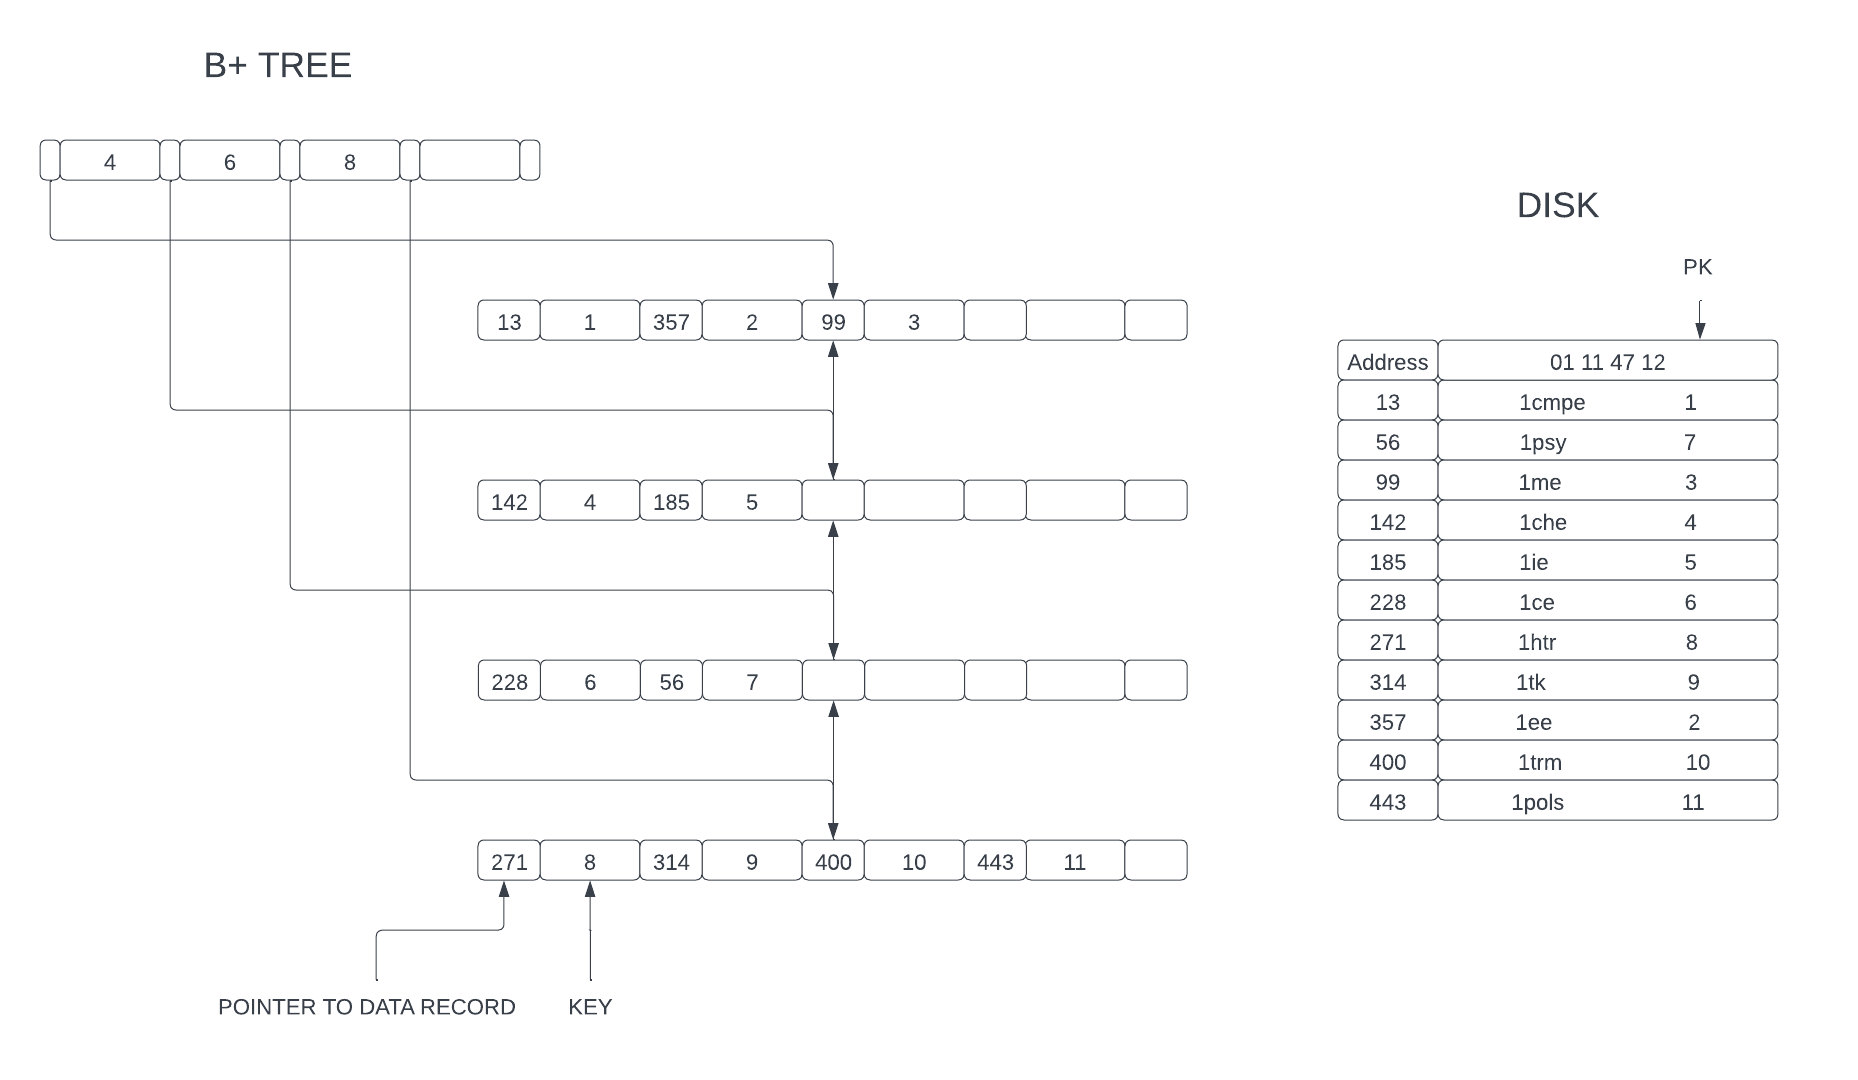
\includegraphics[width=0.9\textwidth]{figures/bplustree.png}
    \caption{An example B+ Tree}
\end{figure}










\section{Operations}
\label{sec:operations}
The implementation of Horadrim consists six python file which perform different parts of the project.

\begin{itemize}
    \item horadrimSoftware.py: the main file of the project which starts the database
    \item sessions.py: the file which helps to preserve the status of the database between sessions
    \item bplustree.py: the file where the B+Tree is implemented
    \item parsing.py: the file reads the input and calls related functions
    \item definition.py: the file performs DDL operations
    \item manipulation.py: the file performs DML operations
\end{itemize}

\subsection{Horadrim Definition Language Operations}
\label{DLL}
The Horadrim Definition Language is a language used to perform operations of types in a database. Required operations are create a type, delete a type and list all types. We implemented these operations in the definition.py file.

\subsubsection{createType(name, no\_fields, pk\_order, fieldHeaders, types, btrees)}
This function is called when the query “create type \textless type-name\textgreater \textless number-of-fields\textgreater \textless primary-key-order\textgreater \textless field1-name\textgreater \textless field1-type\textgreater \textless field2-name\textgreater...” is the input. It first checks if a type with the same name exists. If not, it creates a B+Tree and a new type object with given parameters and updates the System Catalog.

\textbf{Type Object:} Type object enable us to keep the needed information throughout the session. It is created with attributes as name of type, number of fields, field names and types. The specific properties as length of record, residual of a page, maximum number of record per page and maximum number of records per file are calculating after the type is created.

The main usage of type objects is to manage files which has records for that type. It has three important attributes for that purpose.
\begin{itemize}
    \item available: a list which size is equal to number of pages of all files contains the first available location of the page according to index. If no available location in the page, “-1“ for that index.  
    \item no\_records: a list keeps the number of records per page according to index in the current status of storage
    \item files: a list keeps the filenames
\end{itemize}

\subsubsection{deleteType(name, types, btrees)}
This function is called when the query “delete type \textless type-name\textgreater” is the input. It empties the disk memory with deleting the relevant .txt files and deletes the corresponding B+Tree and the saved .json file if exists. It also removes the type object and updates the System Catalog.

\subsubsection{listType(types)}
This function is called when the query “list type” is the input. It lists the all existing types from a list which keeps type objects.

\subsection{Horadrim Manipulation Language Operations}
\label{DML}
The Horadrim Manipulation Language is a language used to perform operations of records in a database. Required operations are create a record, delete a record, update a record, search for a record, list all records of a type and filter the record with a given condition. We implemented these operations in the manipulation.py file.

\subsubsection{createRecord(fields, btrees)}
This function is called when the query “create record \textless type-name\textgreater \textless field1-value\textgreater \textless field2-value\textgreater…” is the input. It first checks if a record with the same primary key exists. If not, it takes the available index with calling the function of the type class, findAvailableIndex(). It writes the record to index which findAvailableIndex() returns. Then, it inserts the [pk, byteaddress] value to the related B+Tree.

\textbf{findAvailableIndex():} This function is implemented to find available locations to write a record to disk. First, it checks the available attribute of the type. If there is an available location, it returns the address of this location. While doing that, it also updates the page headers and the no\_records attribute of type. If the number of records in the page reaches the maximum, available value for that page will be “-1”. Otherwise, the page will be  scanned and the next available location will be stored in available. If there is no available location, it creates either a page or a file and returns the first location in this storage units. 

\subsubsection{deleteRecord(pk, btrees)}
This function is called when the query “delete record \textless type-name\textgreater \textless primary-key\textgreater” is the input. It first searches the address for the given primary key in the B+Tree. Then, it performs the logical deletion operation for the found address. The logical deletion is the process of not actually deleting the record, but setting the record header to “0” to be found by the findAvailableIndex() function. So that, when a new record trying to create, we can overwrite to that index. Also this function checks if the page or file is empty. If they are empty, it deletes.

\subsubsection{updateRecord(pk, fields, btrees)}
This function is called when the query “update record \textless type-name\textgreater \textless primary-key\textgreater \textless field1-value\textgreater \textless field2-value\textgreater...” is the input. It first searches the address for the given primary key in the B+Tree. Then, it overwrites the new field values to that address.

\subsubsection{searchRecord(pk, btrees)}
This function is called by the filterRecord(..) or by the query “search record \textless type-name\textgreater \textless primary-key\textgreater”. It first searches the address for the given primary key in the B+Tree. Then, it reads the record values from that address and returns.

\subsubsection{listRecord(btrees, pk, mode)}
This function is called by the filterRecord(..) or by the query “list record \textless type-name\textgreater”. It has three modes: “0” to list all records, “1” to list records which primary key is bigger than given primary key and “-1” to list records which primary key is smaller than primary key. The function calls the getItems(), getLeft() or getRight() functions of B+Tree according to mode. These functions scan leaf nodes and return ones satisfies the condition. 

\subsubsection{filterRecord(condition, btrees)}
This function is called when the query “filter record \textless type-name\textgreater \textless condition\textgreater” is the input. First, it splits the condition as left-hand side, right-hand side and condition type. Then, it calls one of searchRecord(..) or listRecord(..).

\subsection{Sessions}
\label{sessions}
As a part of the project, inputs will not be independent from each other. So we need to preserve the status of the database between sessions. To handle that, we save the B+Trees are created the session in a .json file with saveTrees() function. When a new session starts, we are deserializing these .json files to load B+Trees with loadTrees() function. The other problem between the sessions is that we can not store Type objects directly. In order to solve this problem, in the beginning of the session, we read the SystemCatalog.txt and scan files. So, we access all the information to create Type objects again.  

\section{Conclusion \& Assessment}
\label{sec:conclusion}
In the project, there were several design choices. One of them was to determine the format of record. In the fixed-length format, all records are exactly the same length in a file. On the other hand, in variable-length records, the length of records varies. We chose the fixed-length records for the types instead of variable-length records. With this choice, we have the advantage of make file processing because the start and end of each record are always a fixed number of characters apart. But, a lot of space is needlessly set aside and wasted.

Another design choice was to select when to save and load the B+Trees. We preferred saving or loading trees when the session is ended or started because saving and loading after every update in tree is a time-consuming process. In large inputs, our design will perform better.


\end{document}
